\documentclass[main.tex]{subfiles} % Subfile-Class

% ============================================================================== %
%                            Subfile document                                    %
% ============================================================================== %

\begin{document}

\subsubsection{Simulation}

Der entwickelte Simulator dient der Visualisierung, Analyse und Optimierung von Algorithmen zur Navigation eines Roboters in einem unbekannten Graphennetzwerk. Er wurde mit dem Ziel konzipiert, eine flexible und intuitive Plattform für die Simulation unterschiedlicher Szenarien zu bieten. Die Funktionen sind so ausgelegt, dass sowohl die interaktive Bedienung als auch automatisierte Simulationen und visuelle Darstellungen unterstützt werden.
Es wurden verschiedene Algorithmen im Simulator implementiert, wie Dijkstra, A* und D*Lite.
Letztendlich hat sich das Informatikteam dafür entschieden, einen eigenen Algorithmus zu entwickeln.
Im Laufe der Entwicklung wurde immer mehr klar, dass es durch das Wegnehmen von Strecken auf dem Graph
zu einem Navigationsproblem kommen kann. Deswegen hat man sich dafür entschieden, nicht mit den Algorithmen
Dijkstra und D*Lite weiterzufahren. Vollständigkeitshalber sind sie aber noch im Simulator enthalten.

\paragraph{Manuelle Bearbeitung von Knoten und Kanten}

Der Simulator erlaubt eine intuitive manuelle Bearbeitung von Knoten und Kanten im Graphen direkt über die Benutzeroberfläche. Dies ermöglicht es dem Nutzer, die Simulation individuell anzupassen und spezifische Szenarien zu testen~\ref{fig:DashboardGraph}:

\begin{itemize}
    \item \textbf{Knoten bearbeiten}:  
    Durch einfaches Klicken auf einen Knoten wird ein Pylon auf diesen gesetzt. Der Pylon repräsentiert ein Hindernis auf dem Knoten. Ein erneutes Klicken entfernt den Pylon wieder, wodurch der Knoten frei wird.

    \item \textbf{Kanten bearbeiten}:  
    Kanten durchlaufen drei Zustände, die durch wiederholtes Klicken in einem zyklischen Ablauf geändert werden können:
    \begin{enumerate}
        \item \textit{Normale Strecke}: Die Kante ist ohne Hindernis befahrbar.
        \item \textit{Entfernte Strecke}: Die Kante wird entfernt, was im UI durch eine gestrichelte Linie angezeigt wird.
        \item \textit{Strecke mit Schranke}: Die Kante ist befahrbar, hat jedoch eine Schranke, die zusätzliche Fahrzeit oder eine andere Einschränkung symbolisiert.
    \end{enumerate}
    Nach einem weiteren Klick kehrt die Kante wieder in den Ausgangszustand als normale Strecke zurück. Dieser Zyklus wird im UI visuell hervorgehoben, um den aktuellen Zustand klar darzustellen.
\end{itemize}

\begin{figure}[H]
    \centering
    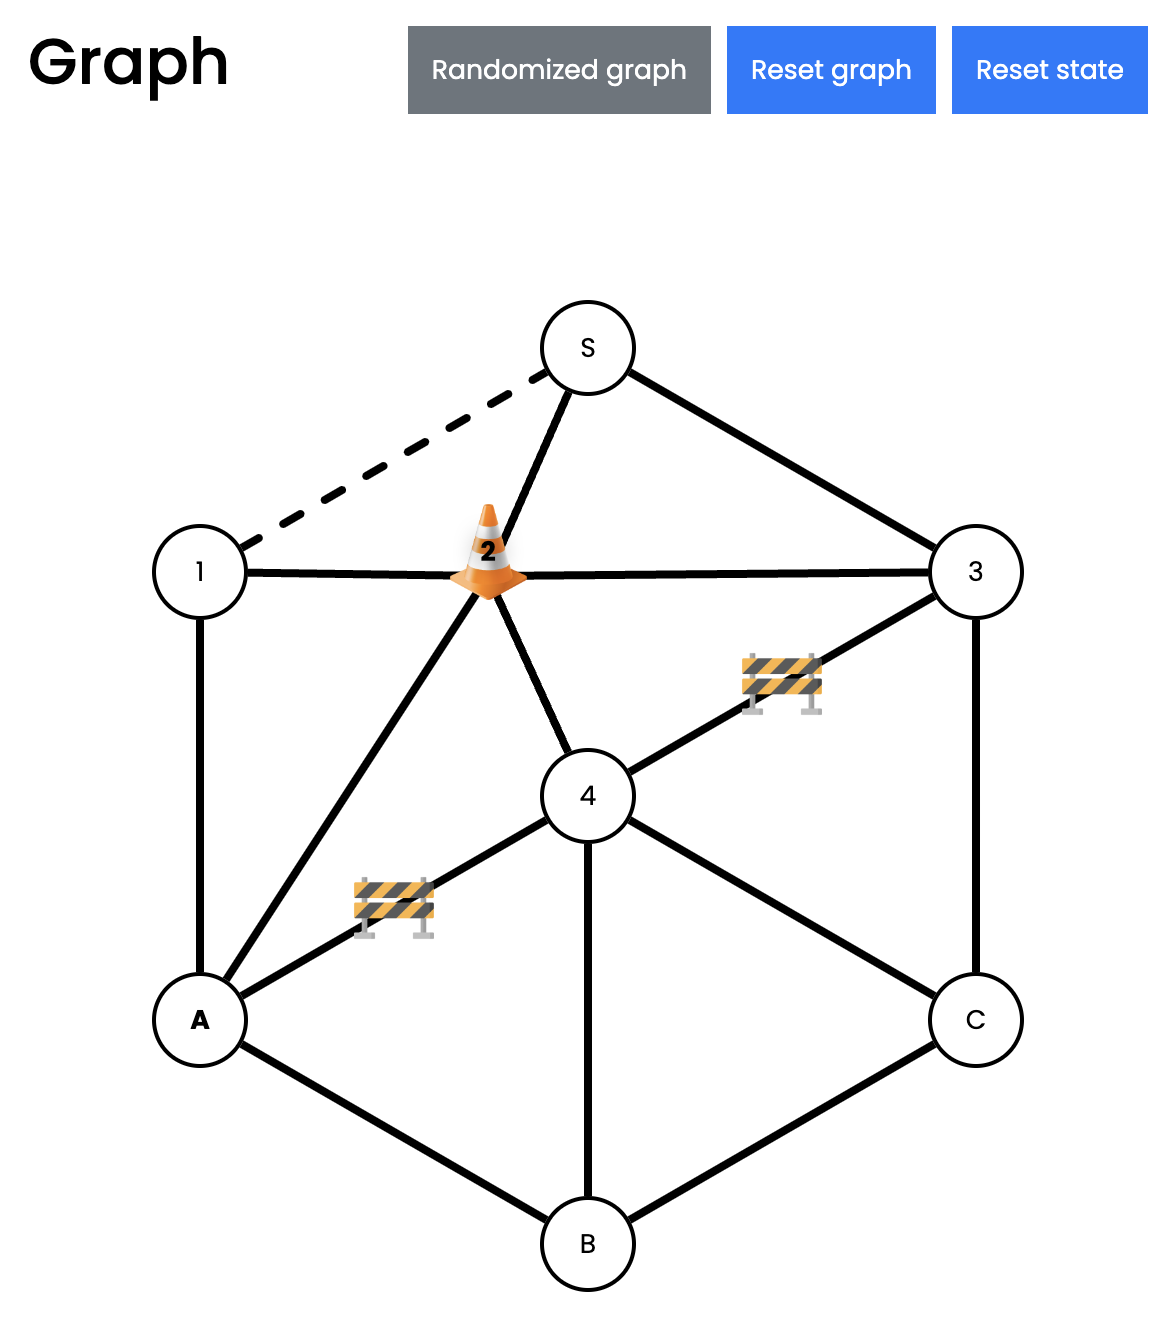
\includegraphics[width=0.75\textwidth]{./fig_Simulation/Graph.png}
    \caption{Section für Graph im Dashboard}~\label{fig:DashboardGraph}
\end{figure}

\paragraph{Visualisierung und Steuerung}

Die Steuerung und Visualisierung des Graphen erfolgt über ein benutzerfreundliches Dashboard. Es stehen drei wesentliche Optionen zur Verfügung~\ref{fig:DashboardGraph}:

\begin{itemize}
    \item \textbf{Randomized Graph}:  
    Generiert einen neuen, zufällig aufgebauten Graphen, der als Grundlage für die Simulation dient.

    \item \textbf{Reset Graph}:  
    Setzt den Graphen in seinen Ursprungszustand zurück, entfernt alle Barrieren, Pylonen und andere Modifikationen.

    \item \textbf{Reset State}:  
    Stellt den Zustand aller Knoten und Kanten auf ihre Standardeinstellungen zurück. Unterschiedliche Stati wie \emph{probed} (gelb), \emph{visited} (grün), \emph{restricted} (rot) oder \emph{finished} (blau) werden visuell hervorgehoben und erlauben eine präzise Nachverfolgung des Algorithmus.
\end{itemize}

Diese Funktionen bieten eine flexible Möglichkeit, den Graphen an spezifische Anforderungen anzupassen und verschiedene Hindernisszenarien zu simulieren.

\paragraph{Funktionen und Modus-Optionen}

Der Simulator bietet drei verschiedene Betriebsmodi. Diese werden durch Tabs voneinander graphisch getrennt~\ref{fig:DashboardConfig}:

\begin{itemize}
    \item \textbf{Interactive run}:
    Dieser Modus erlaubt die interaktive Nutzung des Simulators, wobei spezifische Funktionen und Parameter durch den Benutzer \{tbd!!!!!!\} angepasst werden können.

    \item \textbf{Parameterized run}:  
    In diesem Modus können mehrere Durchläufe automatisiert durchgeführt werden. Es ist möglich, Parameter wie die Fahrzeit auf verschiedenen Strecken (normale Strecken vs. Strecken mit Barrieren), die Anzahl der zu simulierenden Durchläufe (z. B. 100 Runs) und andere Variablen zu spezifizieren. Der Simulator generiert dabei zufällige Graphen und löst diese mittels eines heuristikbasierten Tiefensuchalgorithmus (DFS).

    \item \textbf{Explore Map}:  
    In diesem Modus wird der heuristikbasierte DFS-Algorithmus visuell dargestellt. Der Nutzer kann das Ziel pro Durchlauf selbst bestimmen, wodurch der Graph Schritt für Schritt aufgedeckt wird. Diese Visualisierung identifiziert auch Knoten, die durch mathematische Berechnungen erkannt werden, obwohl der Roboter diese nicht direkt besucht hat. Wenn eine neu entdeckte Kante eine bereits bekannte Kante schneidet, wird anhand linearer Algebra auf die Existenz eines Knotens geschlossen.
\end{itemize}

\begin{figure}[H]
    \centering
    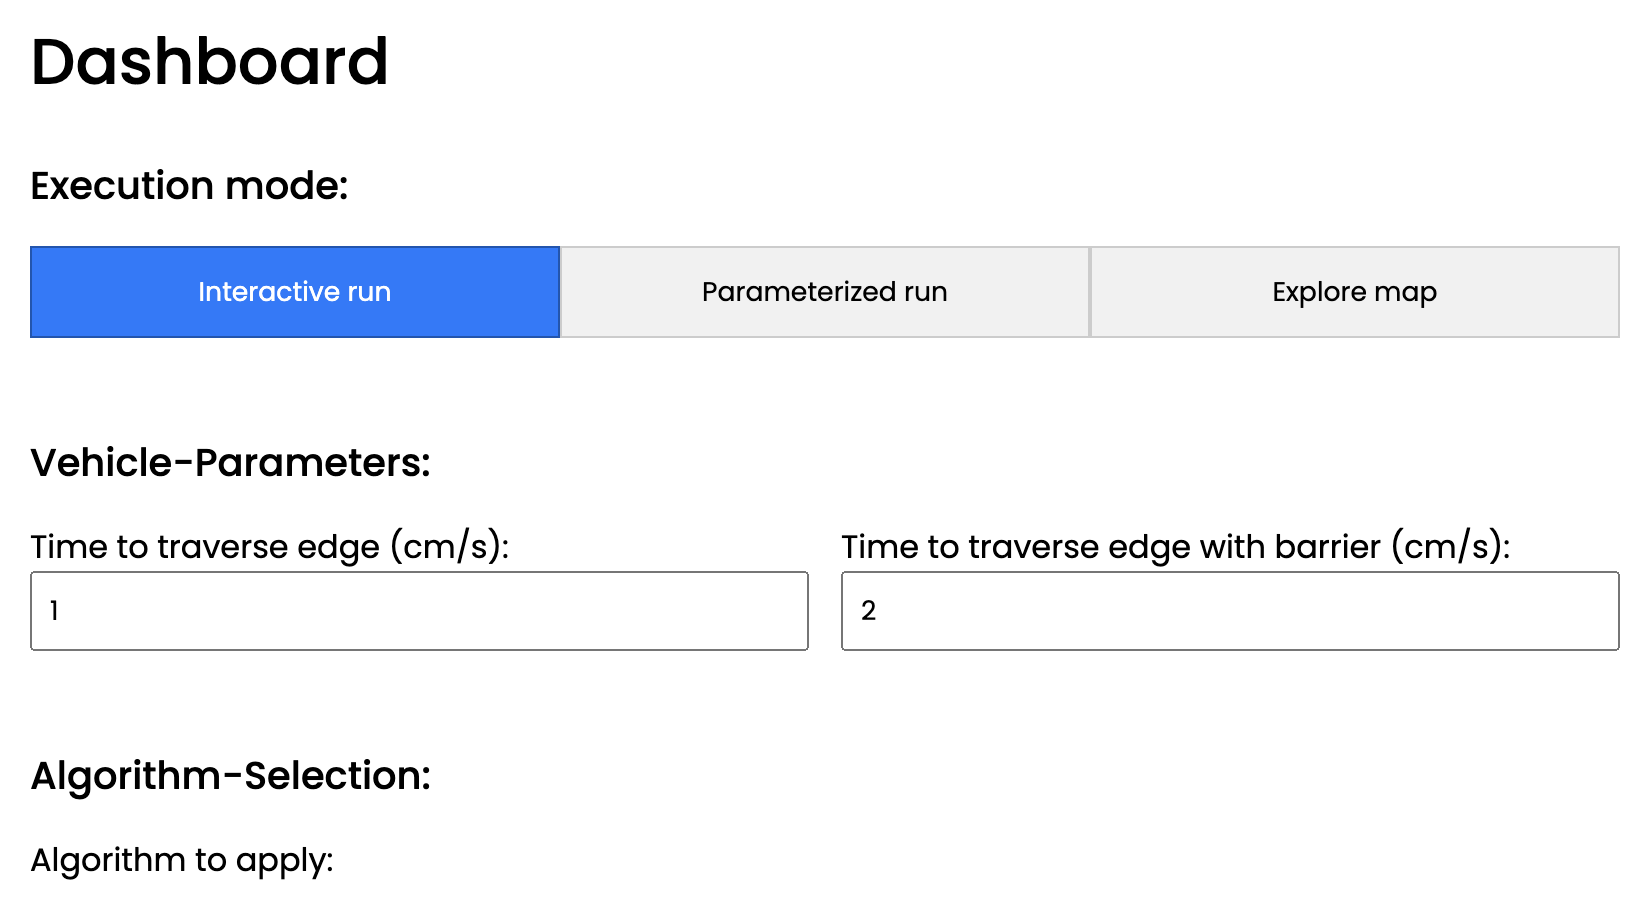
\includegraphics[width=0.75\textwidth]{./fig_Simulation/SimulatorConfig.png}
    \caption{Bereich für Betriebsmodi und deren Konfiguration}~\label{fig:DashboardConfig}
\end{figure}

\paragraph{Log-Analyse}

Der Simulator enthält ein integriertes Log-System, das die Entscheidungen des Algorithmus dokumentiert. Die Logs können direkt im Dashboard gelesen oder als CSV-Datei exportiert werden. Folgende Funktionen stehen zur Verfügung~\ref{fig:DashboardLogs}:

\begin{itemize}
    \item \textbf{Clear Logs}:  
    Setzt die Logs vollständig zurück.

    \item \textbf{Export Logs}:  
    Exportiert die Logs als CSV-Datei.

    \item \textbf{Clear Screen}:  
    Entfernt die Logs aus der Ansicht, ohne diese zu löschen.
\end{itemize}

\begin{figure}[H]
    \centering
    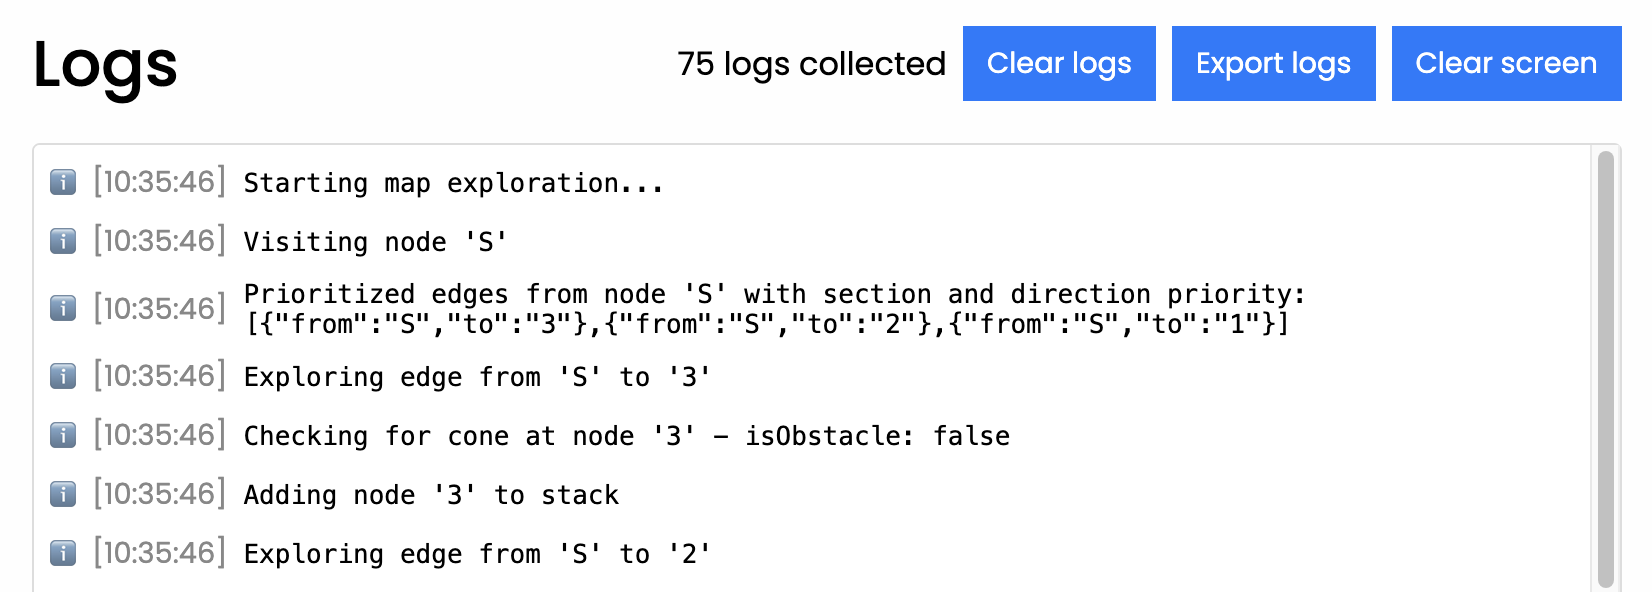
\includegraphics[width=0.75\textwidth]{./fig_Simulation/SimulatorLogs.png}
    \caption{Bereich für Anzeige, Export und Löschung der Logs}~\label{fig:DashboardLogs}
\end{figure}

Die Persistenz der Logs gewährleistet, dass auch nach dem Entfernen vom Bildschirm sämtliche Daten für den Export erhalten bleiben.

\paragraph{Fazit}

Der Simulator bietet eine vielseitige Plattform für die Simulation und Analyse von Navigationsalgorithmen. Durch die Kombination aus visueller Darstellung, flexiblen Betriebsmodi und präzisem Logging ermöglicht er ein umfassendes Verständnis der Funktionsweise und Leistungsfähigkeit der eingesetzten Algorithmen.

\begin{figure}[H]
    \centering
    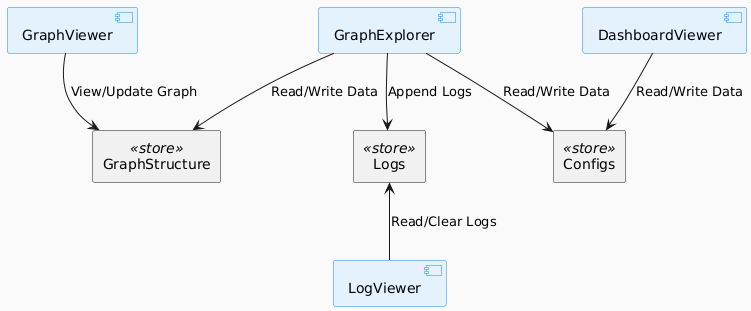
\includegraphics[width=0.75\textwidth]{./fig_Simulation/SimulatorKomponentenDiagramm.png}
    \caption{Aufbau des Simulators und dessen Komponenten}~\label{fig:SimulatorKomponentenDiagramm}
\end{figure}

\end{document}
